
\section*{Etude de la suite logistique}
Nous allons utiliser les fonctions graphiques de Python pour observer quelques particularités de la suite
$\left( x_n \right)_{n\in \mathbb{N}}$ 
définie par la donnée de la valeur $x_0 \in]0,1[$ et de la relation de récurrence : 
$x_{n+1} = \mu x_n\left(1 - x_n\right)$, 
où $\mu$ est une
constante de l’intervalle $\left[0,4\right]$.
On peut visualiser le comportement de ces suites à l’aides de graphes tels ceux tracés en figure suivante, en positionnant l’entier $n$ sur l’axe des abscisses et $x_n$ sur l’axe des ordonnées.

\begin{center}

\includegraphics[width=\linewidth]{fig_01}
\end{center}

Une autre façon de visualiser le comportement asymptotique de la suite $\left( x_n \right)_{n\in \mathbb{N}}$ consiste, à partir des graphes de la
fonction $f_{\mu} : x \mapsto \mu x(1 - x)$ et de la droite d’équation $y = x$, à tracer la ligne brisée reliant les points de coordonnées $(x_0, x_1)$,
$(x_1, x_1)$, $(x_1, x_2)$, ... , $\left(x_{n-1}, x_{n-1}\right)$, $\left(x_{n-1}, x_{n}\right)$ (illustration figure 2).

\begin{center}
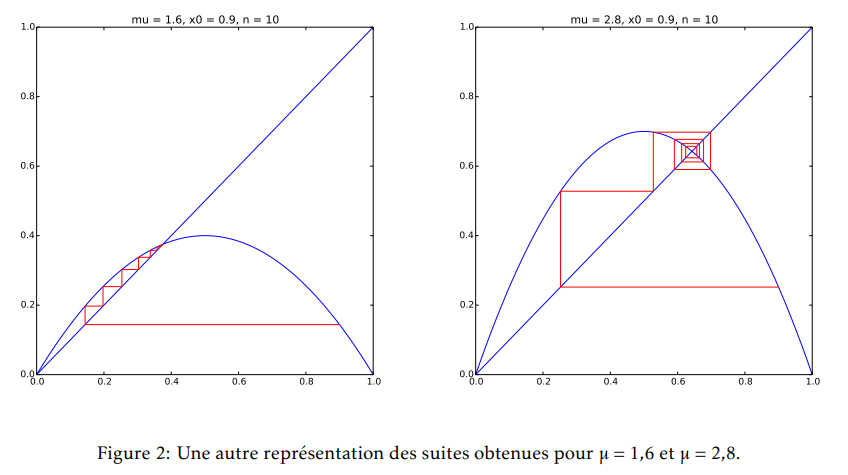
\includegraphics[width=0.8\linewidth]{fig_02}
\end{center}

\subparagraph{}\textit{Définir une fonction \texttt{logistique1(mu, x0, n)} qui permette le tracé des graphes que l’on trouve figure 1, puis une fonction \texttt{logistique2(mu, x0, n)} pour le tracé des graphes de la figure 2.}


\subparagraph{}\textit{À l’aide de ces deux fonctions nous allons (sans démonstration) postuler le comportement de la suite $\left( x_n \right)_{n\in \mathbb{N}}$  en fonction de la valeur de $\mu$. On choisira à chaque fois pour valeur de départ $x_0 = 0,9$ (bien qu’en réalité et mis à part quelques valeurs particulières cette valeur importe peu) et on essayera plusieurs valeurs de $n$.}
\textit{
\begin{enumerate}
\item Lorsque $\mu  \in [0,1]$, observer que la suite $\left( x_n \right)_{n\in \mathbb{N}}$  converge vers 0.
\item Lorsque $\mu  \in [1,3]$, observer que la suite $\left( x_n \right)_{n\in \mathbb{N}}$  converge vers le point fixe $\dfrac{\mu -1}{\mu}$ Quelle différence peut-on faire
suivant que $\mu  \in [1,2]$ ou que $\mu  \in [2,3]$ ?
\item  Lorsque $\mu = 3,05$, qu’observe-t-on ? Et lorsque $\mu = 3,5$ ?
\item Observer enfin la situation pour  $\mu = 3,86$.
\end{enumerate}}

\vspace{.5cm}


Il est possible de démontrer que lorsque µ est compris entre 3 et $1+\sqrt{6}$ (environ 3,45) la suite $\left( x_n \right)_{n\in \mathbb{N}}$  finit par osciller entre deux valeurs dépendantes de $\mu$ mais pas de $x_0$. Entre 3,45 et (environ) 3,54 la suite finit par osciller entre quatre
valeurs. au delà de cette valeur la suite oscille entre huit valeurs, puis seize, etc. À partir de d’environ 3,57, le chaos
s’installe et mis à part certaines valeurs il n’est plus possible de décrire le comportement asymptotique de la suite.
Tout ceci peut être résumé par le diagramme des bifurcations : l’axe des abscisses porte les valeurs du paramètre $\mu$, l’axe des
ordonnées les valeurs d’adhérences possibles.


\begin{center}
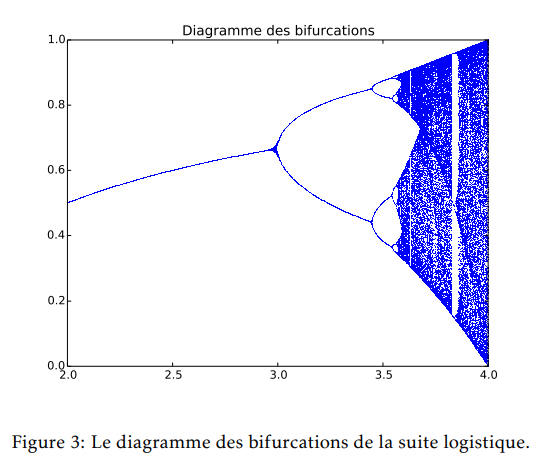
\includegraphics[width=0.6\linewidth]{fig_03}
\end{center}


\subparagraph{}\textit{Le diagramme des bifurcations de la figure 3 a été obtenu en faisant varier $\mu$ entre 2 et 4 avec un pas égal à 0,002. Pour chacune des valeurs de µ sont représentées en ordonnée les valeurs distinctes à $10^{-3}$ près de $x_{101}$, $x_{102}$,..., $x_{200}$.Le tracé a été obtenu avec les options \texttt{marker=','}, \texttt{linestyle=''}. Rédiger un script Python qui réalise le tracé de ce diagramme.}


\subsection*{Exposant de Lyapunov}

Le système dynamique obtenu pour $\mu = 4$ est chaotique : une infime variation de la valeur initiale $x_0$ modifie du tout
au tout la valeur de  $x_n$ après seulement quelques itérations. Pour mesurer l’influence d’un écart $e_0$ sur $x_0$ pour la suite
 $\left( x_n \right)_{n\in \mathbb{N}}$ on calcule l’écart absolu après une itération : $e_1 = f_{\mu}(x_0 + e_0) - f_{\mu}(x_0)$. L’écart relatif vaut $\dfrac{|e_1|}{|e_0|}=\left| \dfrac{f_{\mu}\left( x_0 +e_0\right)-f_{\mu}\left(x_0\right) }{e_0} \right|$,  quantité que l'on appproche $\left| f'_{\mu}\left( x_0\right) \right|$ sachant que $e_0$ est petit. Après $n$ itérations l'écart relatif vaut donc : 
$$
\dfrac{|e_n|}{|e_0|} =\dfrac{|e_n|}{\left| e_{n-1} \right|} \times ... \times \dfrac{|e_1|}{\left| e_{0} \right|} \simeq \prod \limits_{k=0}^{n-1} \left| f'_{\mu}\left(x_k\right)\right|.
$$

Notre objectif est de déterminer si les écarts s’amplifient et donc si ce produit est supérieur à 1 ou si le système est stable
et le produit inférieur à 1. Sachant que réaliser une addition est plus rapide qu’une multiplication, on étudie plutôt le
logarithme de cette quantité :

$$
\prod \limits_{k=0}^{n-1} \left| f'\left(x_k\right)\right|<1 
\Leftrightarrow
\sum \limits_{k=0}^{n-1} \ln \left| f'_{\mu}  \left(x_k\right)\right|<0 
$$

et pour relativiser le rôle du choix de n on divise cette somme par $n$.
Ceci conduit à définir l’exposant de Lyapunov :

$$\lambda_ {\mu} =  \lim\limits_{n\to +\infty}\dfrac{1}{n} \sum_{k=0}^{n-1} \ln \left| f'_{\mu}  \left(x_k\right)\right| .$$

\subparagraph{}\textit{Rédiger une fonction \texttt{lyapunov(mu, x0, n)} qui calcule une approximation de cette quantité en fonction
de la valeur de $\mu$, de $x_0$ et du nombre d’itérations $n$ choisi.
Tracer ensuite le graphe représentant les variations de $\lambda_{\mu}$ en fonction de $\mu$ dans l’intervalle $[3,4]$ à partir de la valeur $x_0 = 0,9$. Comment interpréter ce graphique ?}

\begin{center}
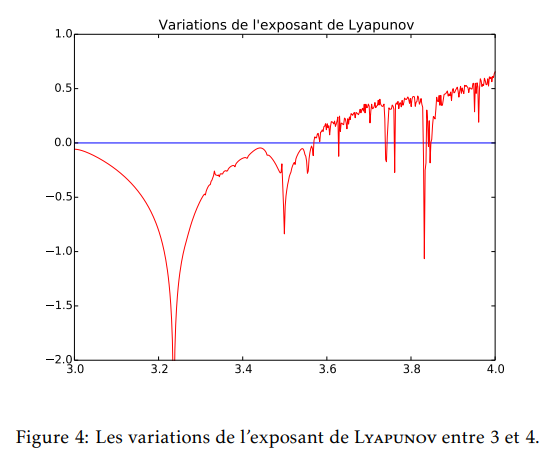
\includegraphics[width=0.6\linewidth]{fig_04}
\end{center}


Observons de nouveau le diagramme des bifurcations. Pour $\mu_0 = 3$ a lieu la première bifurcation ; pour $\mu_1 = \simeq 3,45$ a lieu la seconde. Plus généralement on note $\mu_k$ la valeur de $\mu$ où a lieu la $(k + 1)$\ieme bifurcation. La constante de Feigenbaum est la valeur de la limite :
$$
\delta = \lim_{n \to \infty} \dfrac{\mu_{n+1}-\mu_{n}}{\mu_{n+2}-\mu_{n+1}}
$$

\subparagraph{}\textit{Essayer d’obtenir une approximation de cette constante (pour information on a $\delta = 4,669 201...$).}


Indication. Pour déterminer la taille du cycle limite, définir une fonction qui calcule le nombre de valeurs distinctes à $10^{-4}$ près des termes $x_{n+1}$,..., $x_{n+256}$ pour une grande valeur de $n$ (par exemple 100 000). En procédant à des recherches
dichotomiques déterminer les six premières bifurcations et calculer $\dfrac{\mu_5-\mu_4}{\mu_6-\mu_5}$.

Remarque. Cette constante a ceci de remarquable qu’on la retrouve dans d’autres diagrammes des bifurcations, par
exemple en étudiant les suites définies par la relation de récurrence $x_{n+1} = \mu\sin(x_n)$ ou encore $x_{n+1} = \mu  - x_n^2$. Si vous en avez le temps vous pouvez mettre en évidence son caractère universel en reprenant votre étude avec l’une ou l’autre de ces
deux relations.
